\chapter{Software design}

\label{ch:Software design}

\setlength{\parindent}{4em}
\setlength{\parskip}{1em}
\renewcommand{\baselinestretch}{1.5}

\section{System architecture}

\subsection{System architecture}
\hspace{1.5cm}In our project, we use two algorithms to stimulate the subject. First use ERPs which is different in stimulating time. Second is SSVEP which difference in stimulating frequency.

\begin{figure}[h]
	\centering
	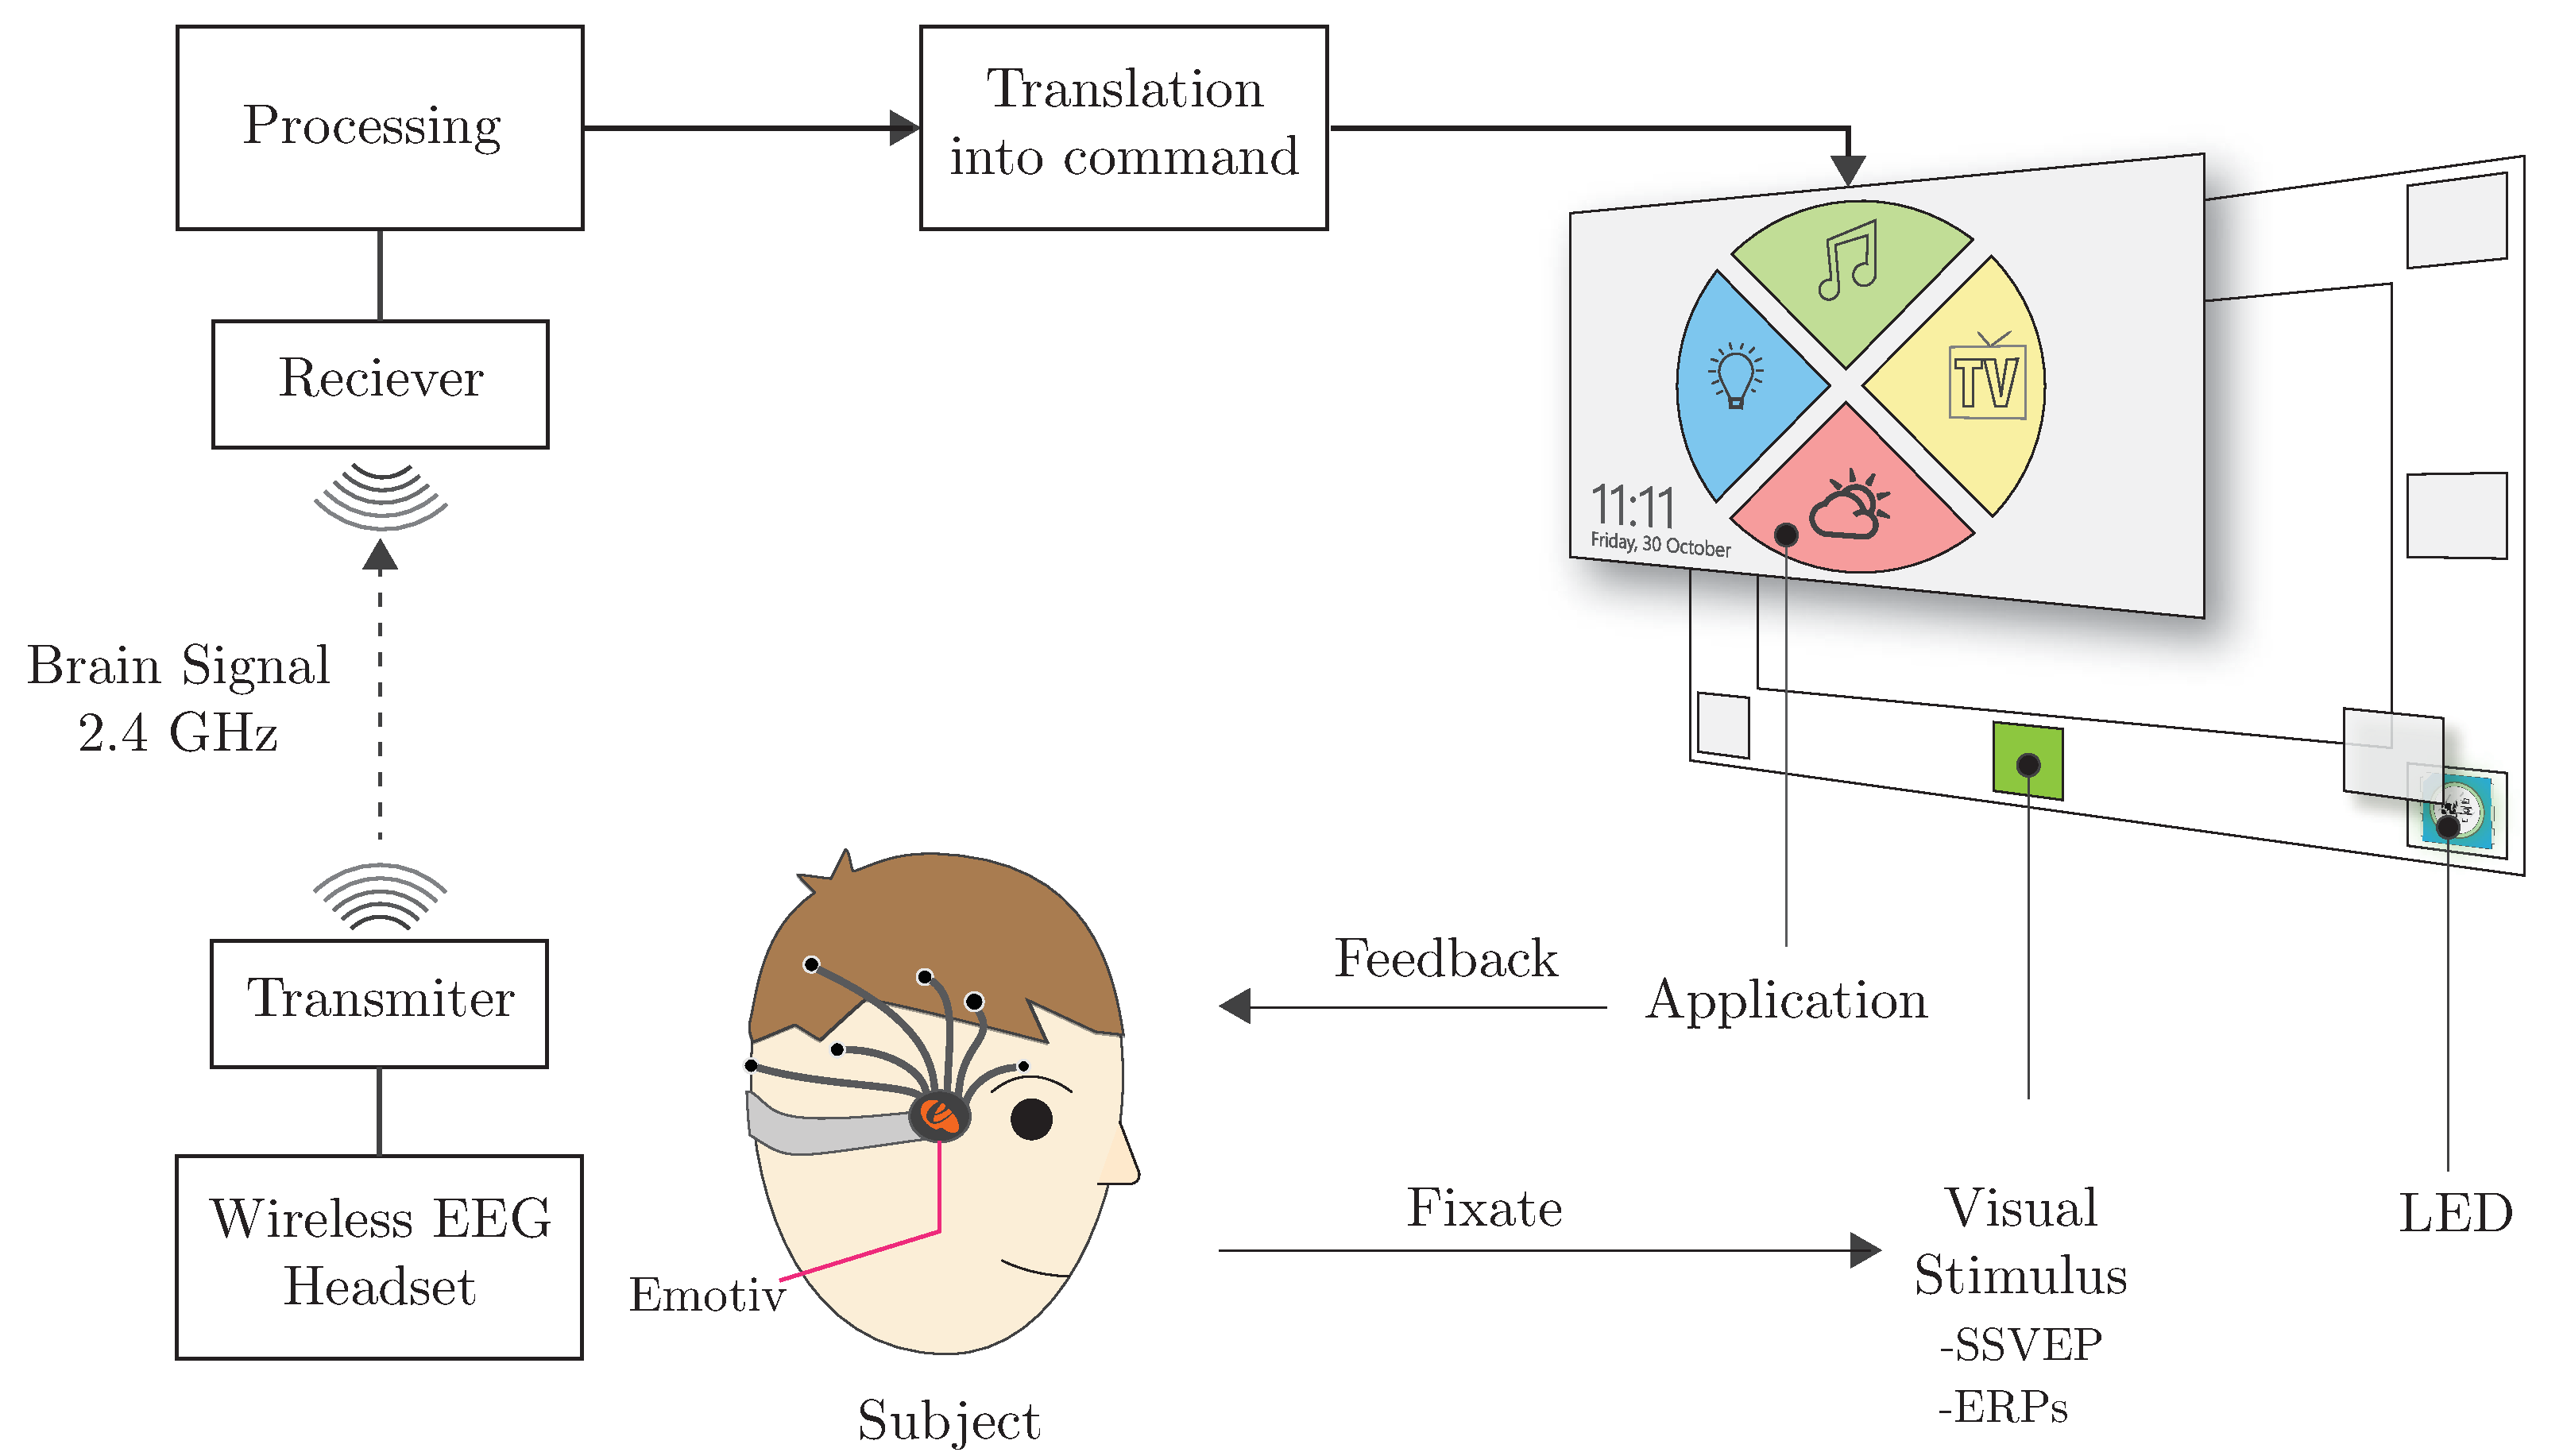
\includegraphics[scale = 0.3]{chapter5/architec.pdf}
	\caption{System architecture design}
\end{figure}

\subsection{Class Diagram}

\begin{figure}[h]
	\centering
	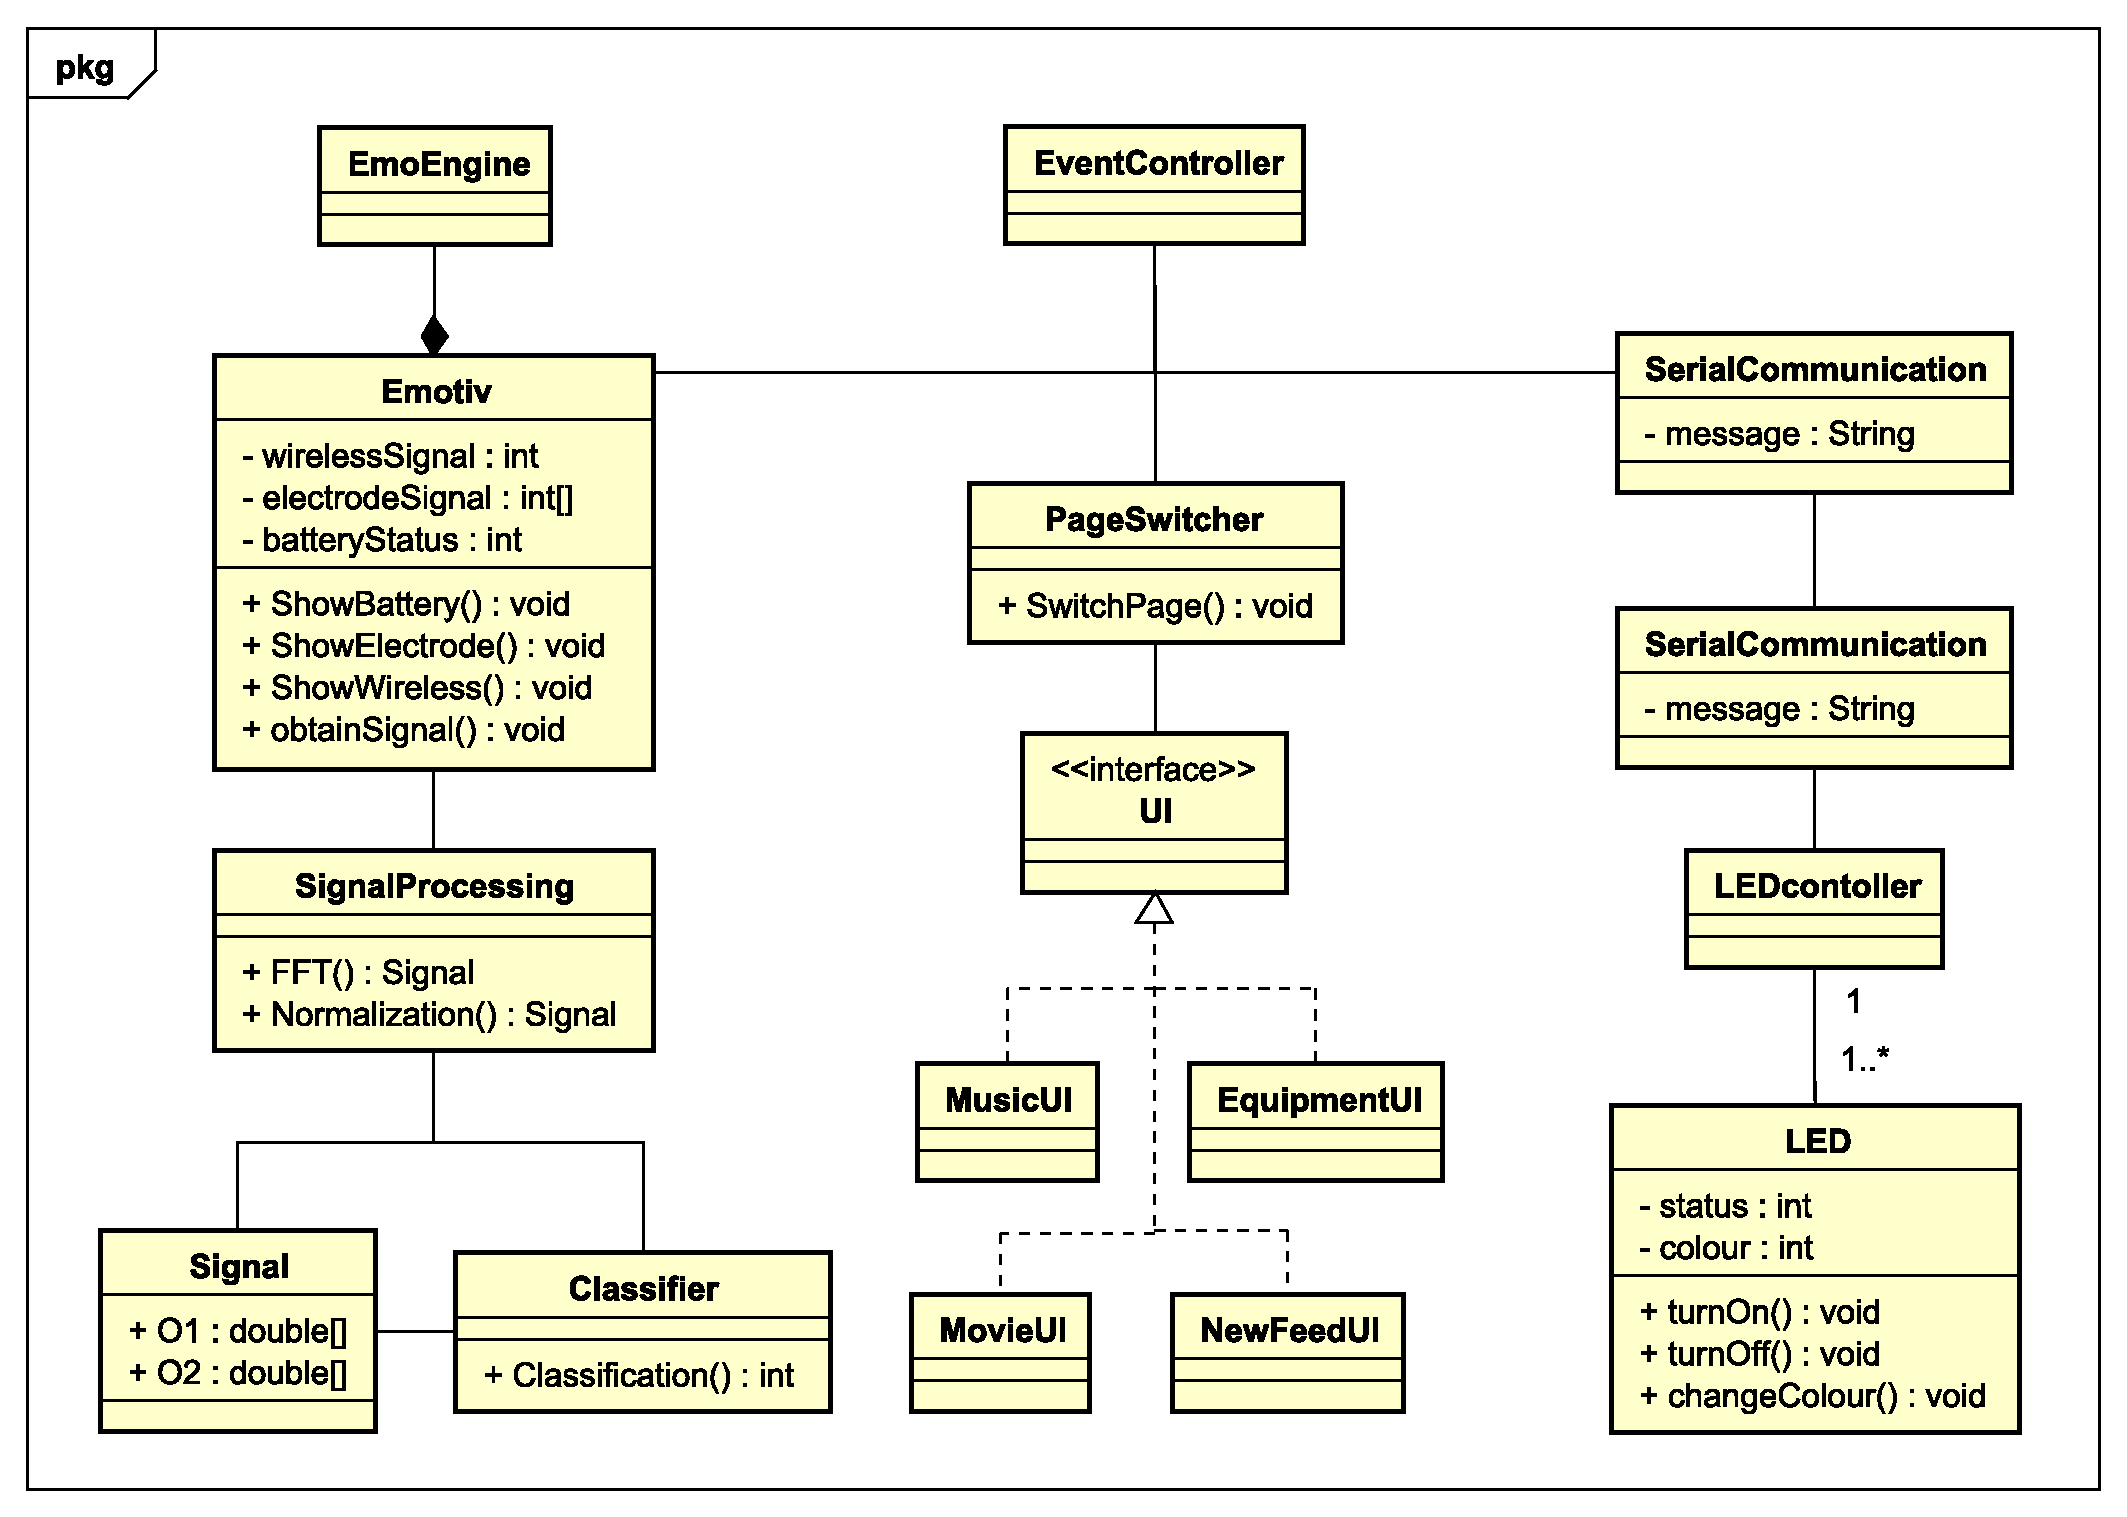
\includegraphics[scale = 0.5]{chapter5/Class.pdf}
	\caption{Class diagram}
\end{figure}

class diagram description